% !TeX program = xelatex
\documentclass[a4paper, 12pt]{article}

\usepackage[table]{xcolor}
\usepackage[top=8mm, bottom=8mm, left=18mm, right=18mm,
            headsep=6mm,
            headheight=40pt,
            includeheadfoot,
            bindingoffset=0mm]{geometry}
\renewcommand{\baselinestretch}{1.2}

\usepackage{hyperref}
\usepackage{tikz}

% ---CUSTOMISE ENUMERATION--- %
\usepackage{enumitem}

% ---FOR LANDSCAPE ORIENTED PAGES--- %
% \usepackage{lscape}

% ---ABSOLUTE TEXT POSITIONS--- %
\usepackage[absolute,overlay]{textpos}

% ---USE DIFFERENT FONTS--- %
% Uncomment the following 2 lines if you wanna use tetex and ...
%\usepackage{fontspec}
%\newfontfamily\headerfont{TeX Gyre Heros Bold}
% ... comment out this definition command "headerfont" which says to do nothing:
\newcommand{\headerfont}{}

% ---MATH AND EQUATION PACKAGES--- %
% \usepackage{amsmath, amssymb}
% \DeclareMathOperator{\sign}{sgn}
% \newcommand*\diff{\mathop{}\!\mathrm{d}}
% \usepackage{siunitx}

% ---SHADED TEXT AND TEXT COLOR--- %
% \usepackage{framed}
 \usepackage{xcolor}
 \definecolor{iwtdark}{HTML}{9d3238}
 \definecolor{iwtlight}{HTML}{cd8d25}
 \colorlet{shadecolor}{iwtlight!25}

% ---CHANGE PAGE HEADERS--- %
\usepackage{fancyhdr}
\usepackage{xpatch}
\xpretocmd\headrule{\color{lightgray}}{}{\PatchFailed}
\renewcommand{\headrulewidth}{0.6mm}% 2pt header rule
\fancyhf{} % sets both header and footer to nothing
\fancyhead[L]{
    \headerfont\scriptsize
    \textcolor{iwtdark}{
      Data Management Guidelines: \\
      How To Handle Data
    }
    \vfill
}
\fancyhead[R]{
 \includegraphics[height=12mm]{Figure00_IWT-Logo.png}
}
\fancyfoot[C]{\headerfont\fontseries{bx}\textcolor{iwtdark}{\thepage}}
\fancypagestyle{plain}{
   \fancyhf{} % sets both header and footer to nothing
   \fancyfoot[CO, CE]{\headerfont\fontseries{bx}\textcolor{iwtdark}{\thepage}}
}
\pagestyle{fancy}

% ---CHANGE HEADING LAYOUT--- %
\usepackage{titlesec}
\titleformat{\section}[hang]%
  {\normalfont\fontseries{bx}}%
  {\headerfont\Large\fontseries{bx}\color{iwtdark}\thesection}%
  {1em}{\headerfont\fontseries{bx}\Large\color{iwtdark}}

\titleformat{\subsection}[hang]%
  {\normalfont\fontseries{bx}}%
  {\headerfont\large\fontseries{bx}\color{iwtdark}\thesubsection}%
  {1em}{\headerfont\fontseries{bx}\large\color{iwtdark}}

\titleformat{\subsubsection}[hang]%
  {\normalfont\fontseries{bx}}%
  {\headerfont\fontseries{bx}\color{iwtdark}\thesubsubsection}%
  {1em}{\headerfont\fontseries{bx}\color{iwtdark}}

\titleformat{\paragraph}[hang]%
  {\normalfont\normalsize\bfseries}%
  {\theparagraph}%
  {1em}{\headerfont\normalsize\bfseries\color{iwtdark}}

% ---INCLUDE FIGURES--- %
\usepackage{graphicx}
\graphicspath{{../../02_Figures/}}
\usepackage[font=small,labelfont=bf,justification=justified,
            singlelinecheck=false]{caption}
\usepackage{subcaption}
\usepackage{wrapfig}

% ---CHANGE TABLE LAYOUT--- %
\usepackage{booktabs}
\usepackage{makecell}
\usepackage{tabularx}
\usepackage{multirow}

% ---AUTOMATED BIBLIOGRAPHY--- %
\usepackage{biblatex}
\addbibresource{../../06_References/references.bib}
\usepackage{csquotes}

% ---INCLUDE PDFS--- %
% \usepackage{pdfpages}

% ---PSEUDOCODE --- %
% \usepackage{algorithm}
% \usepackage[noend]{algpseudocode}
% \makeatletter
% \def\BState{\State\hskip-\ALG@thistlm}
% \makeatother

\usepackage[USenglish]{babel}

\usepackage{todonotes}

%Table usepackages
\usepackage[table]{xcolor}
\usepackage{tabularx}
\usepackage{booktabs}
\usepackage{array}

\usepackage{caption}

%\renewcommand{\rmdefault}{phv} % Arial
%\renewcommand{\sfdefault}{phv} % Arial
\usepackage{fontspec}
\setmainfont{Liberation Sans}

\usepackage{float}

%for dashed lines in tables:
%\usepackage{arydshln}
\providecommand{\hdashline}{\hline}
%\usepackage{glossaries}
%\makeglossaries

% ---CUSTOM COMMANDS--- %
\newcommand{\tabitem}{~~\llap{\textbullet}~~}
\newcommand{\documenttitle}{Data Management Guidelines:\\ How To Handle Data}

\newcommand{\documentauthor}{Norbert Riefler}

\title{\documenttitle}
\begin{document}

\begin{titlepage}
  %\includepdf[pages=-]{figures/Titlepage.pdf}
  \tikz[remember picture,overlay] \node[opacity=1.0,inner sep=0pt] at (current page.center){
\includegraphics[width=1.05\paperwidth,height=1.05\paperheight]{Figure00_Titlepage_Background.pdf}};
  \begin{textblock*}{10cm}(1.5cm,16cm) % {block width} (xcoord, ycoord)
    \noindent
    \raggedright
    \textcolor{white}{
      \Huge\headerfont\fontseries{m}\documenttitle \\
      \vspace{6cm}
      \large\today
    }
  \end{textblock*}
  \begin{textblock*}{5cm}(15.4cm,28.5cm)
    \noindent
    \raggedright
    \textcolor{white}{
      \large\headerfont\fontseries{bx}\documentauthor
    }
  \end{textblock*}
\end{titlepage}
\newpage
\thispagestyle{empty}
\begin{center}
  \large\headerfont\fontseries{m}\textcolor{iwtdark}{Preface}
\end{center}

\begin{quote}
  `On July 20, 1969, Neil Armstrong climbed out of his spacecraft and
  placed his feet on the moon. The landing was broadcast live all over the
  world and was a significant event in both scientific and human History.
  Today, we can still watch the grainy video of the moon landing but what we
  cannot do is watch the original, higher quality footage or examine some of
  the data from this mission. This is because much of the data from early space
  exploration is lost forever. (...) The tapes were likely wiped and reused for
  data storage sometime in the 1970s.' \\
  \null\hfill - \citeauthor{briney2015}\cite{briney2015}
\end{quote}

\noindent This reader (https://github.com/Leibniz-IWT/DataManagementGuidelines) holds for all employees of the Leibniz-Institute for Materials Engineering (IWT) and serves as a reference
for how to save data. It delivers reasons for the question of why one should
think about data management and gives instructions and examples. Data management
in the information age is an absolutely required skill and a base to cope with
the wealth of data to avoid an information overload. It helps organizing
everyone’s own data, but it is also mandatory for data sharing so that others
can understand the structure and are able to interpret the information given by
your data. In this way, your data meet the FAIR standard (Findable, Accessible,
Interoperable and Reusable), basis for the new discipline of data science.

There are many topics in data management like data governance and security or
storage management, but we are treating here only a condensed extract, tailored
to data handling in our department. Therefore, this reader might help you to
clarify what must be done to be a data steward, and it follows the guidelines given by the Leibniz Association \cite{leibniz2018}.
\newpage

\tableofcontents      
% \listoffigures
% \listoftables
\newpage
\section{Why Data Management}

\textbf{Save time} \\
Planning your data management will save you time and resources \cite{martinez-garcia:2023:Heliyon}, e.g., by faster locating data. And well managed data requires less preparation for sharing or writing a paper. \\[6pt]
\textbf{Preserve your data} \\
Depositing your data in a file server (repository) safeguards your investment of time and resources while preserving your research contribution for you and others to use. \\[6pt]
\textbf{Increase your research impact} \\
Making your data available to other researchers can impact discovery and relevance of your research. \\[6pt]
\textbf{Maintain data integrity} \\
Managing and documenting your data throughout its life cycle will allow you and others to understand and use your data in the future. \\[6pt]
\textbf{Meet grant requirements} \\
Many funding bodies now require that researchers deposit data collected as part of a research project. \\[6pt]
\textbf{Promote new discoveries} \\
Sharing your data with other researchers can lead to new and unanticipated discoveries and provide research material for those with little or no funding. \\[6pt]
\textbf{Support open access} \\
Be a catalyst for research and discovery. Show your support for open access by sharing your data.

%\section{Data Management Plans}

The handling of the data, created during a project, contains several issues
which are described in a Data Management Plan (DMP). A DMP contains structured
information about the research process of the corresponding project. But these
information has to be given long before a project is started: Applicants have
to create a DMP in every proposal, required by all important research funding
organizations (DFG, BMBF, etc.). So in the process of writing, applicants start
to think about how they will treat data. The following topics belongs to typical
DMPs and might be of interest to you; more details can be found in
\cite{dfg2021,hannover2020}:
\begin{enumerate}
  \item Administrative information: project name, kind of funding, time period.
  \item Methods of data generation: simulations, experiments (devices),
        data size, kind of data documentation.
  \item Data safety: location, interval and capacity of storage device,
        who gets access.
  \item Archiving: which data are archived where with what kinds of metadata.
  \item Data sharing: which repository, license condition, required metadata.
  \item Resources and responsibility: who is responsible for processes, IT,
        defining defaults and formats, monitoring; required personal resources;
        costs.
\end{enumerate}
Please see \cite{dfg2021,hannover2020} and the Appendix for more details; some exemplary DMPs can be found here:
\url{https://www.cms.hu-berlin.de/de/dl/dataman/arbeiten/dmp_erstellen}

\section{File Organization}
The following explains what and how to save your files on our servers:
\begin{itemize}
  \item Access to the Server of Process Engineering department (VT) is established with your Web browser by entering the web address in the address field, via mapping the VT-Server to the Windows Explorer as an own drive, or by using the Synology Drive Client (see \cite{synology2022}) with some more and very helpful options like, e.g., document versioning. The \textbf{maximum size} of uploaded data should not exceed \textbf{100Gbyte per file}. Access privilege is administrated by Stefan Endres (\href{mailto:s.endres@iwt.uni-bremen.de}{s.endres@iwt.uni-bremen.de}) and Nils Ellendt (\href{mailto:ellendt@iwt.uni-bremen.de}{ellendt@iwt.uni-bremen.de}).
  \item The server of the Manufacturing Technology (FT), Materials Engineering (WT) and Institute of Materials Testing (MPA) are accessed via browser or windows explorer. Access privilege is administrated by the IWT IT division.
\end{itemize}

\subsection{Different Data Types and Storage Strategy of Large Data}
Depending on the origin of the data, we distinguish between two data types \cite{gitelman2013}:
\begin{itemize}
  \item Primary data (sometimes called raw data) is generated by measurement
        devices, sensors/cameras, simulation programs, observations etc. and
        are untreated; it is collected for the first time by the researcher.
  \item Secondary (or analyzed) data are processed primary data. (In social
        science, secondary data are already collected or produced data by
        others).
\end{itemize}
Data from projects are stored in the according project directory. All experiments and simulations documented in the ELN get an ELN protocol as PDF which are also saved in this directory. Very large primary data cannot be stored in the ELN. However, the origin and the storage location (e.g. the precise location on the file server) of these data can be documented there. The rules are:






\begin{itemize}
  \item data $<$ 100 MByte is stored and documented on the ELN
  \item all data $>$ 100 MByte is stored on the file server and documented
        in the ELN.
\end{itemize}
High-speed video movies can be highly compressed and stored as a mp4-file and uploaded to the ELN instead of the primary data.

Large amount of data needs specific care; see for instance the 10$^{th}$ rule of Hart et al. \cite{hart:2016:PLOSComputBiol}. Depending on the amount of the data, there are different storage strategies shown in figure \ref{fig:storage-strategy}.

\begin{figure}[H]
  \vspace{-1em}
  %Das yEd-File ist hier: /home/riefler/Daten/0/Wissenschaft/Uni+IWT/Computing/IWT-EDV/EDV-Struktur/IT-Ausschuss/DataStorageStrategy-Unterausschuss
  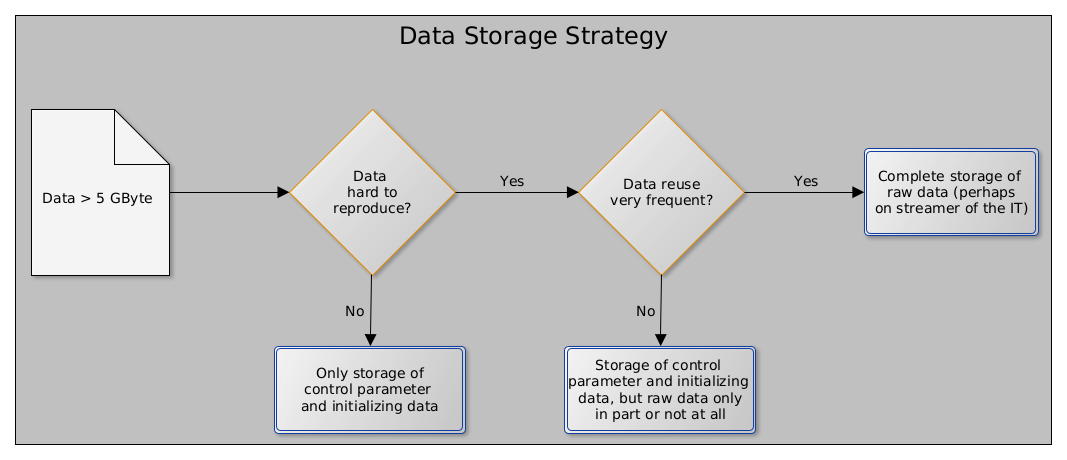
\includegraphics[width=\linewidth]{Figure01_DataStorageStrategy-Englisch.png}
%  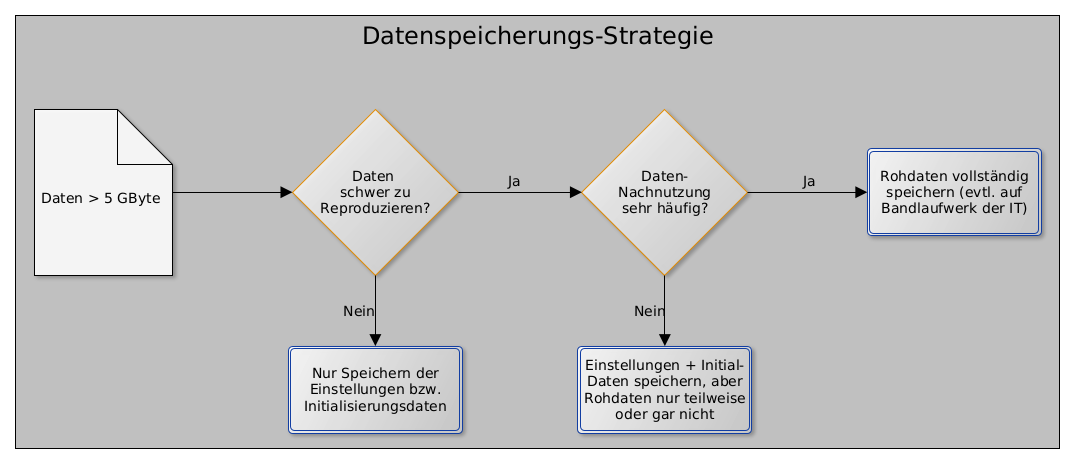
\includegraphics[width=18cm]{Figure01_DataStorageStrategy-Deutsch.png}
  \caption{Pfade der Speicher-Strategie}
  \label{fig:storage-strategy}
\end{figure}
Most important for the strategy is to consider the expense of the reproduction of the data. Simulations can be easily repeated as long as all input parameter, the complete software package and the underlying operating system is stored. However, complex experiments cannot be reproduced that easy. Therefore, large amount of data from experiments are in principle assesed to be more valuable as data from simulations. The generation of data for one transient simulation using High Performance Computing (HPC), e.g. using the NHR (Nationale Hochleistungsrechner), often exceeds 1 TByte. The storage of these data should be in accordance to the IWT IT either on a fileserver or an USB hard drives, and the content of the data is documented on the ELN.

The storage period of data is limited to 10 years. Afterwards, the data will be deleted by the IWT IT. The responsible person of theses data (i.e. the department leader) get a message six month before. If she or he reply still needs the data, they can be stored for a determined time. Data of publications (subdirectory 'Publications' under the project directory) persists unless they are stored on a repository (for instance on zenodo.org), with a remark and link to that repository to retrieve the data.

It is absolutely necessary to \textbf{check all data from external sources} (e.g. from an USB stick) manually against computer viruses before usage or storage of the data. Above that, data loss is common on USB sticks if they are not used over a longer time span, so they should never used for data storage.


\subsection{File and Folder Naming}

Spend time planning out file naming conventions in the beginning of a project. How do you or others will look for and access files at a later date? Do you think about them by type, location, study or something else? \\[8pt]
Naming conventions:
\begin{itemize}
  \item File names are self-explanatory - they tell what data is in!
  \item Do not use spaces or special characters - use CamelCase and hyphen
        ‘-’ or underscore ‘\_’ as separator: \\
        \begin{tabular}{ll}
          \textcolor{red}{\textbf{NO}}  & \textcolor{red}{‘name date v1.txt’} \\
          \textbf{YES} & ‘name\_date\_v01.txt’ \\
          \textbf{YES} & ‘nameDateV01.txt’ \\
          \textbf{YES} & ‘simpleFoam\_u0.2m-s\_etha2mPas\_v01’ \\
        \end{tabular}
  \item Develop a file naming scheme that includes information about the data.
        Example: \\
        {[Date]}\_{[Run]}\_{[SampleType]}
  \item Consider sorting when deciding what element of the file name will
        go first: \\
        Use ‘YYYY-MM-DD’ to save dates. \\
        Use leading zeros: \\
        \begin{tabular}{lll}
          \textcolor{red}{\textbf{NO}}  & ‘ProjID\_v1.csv’  	...  	\textcolor{red}{‘ProjID\_v11.csv’} & \\
          \textbf{YES} & ‘ProjID\_v01.csv’ 	... 	‘ProjID\_v11.csv’
             & (sequence up to 99) \\
          \textbf{YES} & ‘ProjID\_v001.csv’ 	...	‘ProjID\_v111.csv’
             & (sequence up to 999) \\
        \end{tabular}
\end{itemize}

\subsection{File Formats}
As technologies change, researchers should plan for both hardware and software obsolescence and consider the longevity of their file format choices to ensure long term readability and access.


File formats more likely to be accessible in the future have the following characteristics:
\begin{itemize}
  \item Non-proprietary
  \item Open, documented standard
  \item Common usage by research community
  \item Standard representation (ASCII, Unicode)
  \item Unencrypted
  \item Uncompressed (if not too large...)
\end{itemize}

\noindent Examples of \textbf{preferred} file format choices include:
\begin{itemize}
  \item Open Document Files: .odt (Text), .ods (Spreadsheet),
        .odp (Presentation); primary format of OpenOffice/Libre Office,
        standardized in ISO 26300
  \item Office Open XML: .docx (Text), .xlsx (Spreadsheet),
        .pptx (Presentation); primary format of Microsoft Office,
        standardized in ISO 29500
  \item Ritch Text Format: .rtf; proprietary, but well documented format
  \item Plain Text or Markup Language: .txt, .md (Markdown), .html (Hypertext),
       .tex (LaTeX), .csv (comma separated values)
  \item Portable Document Format: .pdf; standardized in ISO 32000
  \item Bibliographic Data: .enl (EndNote; this is the standard software for
        literature management at the IWT); otherwise, please use human readable
        formats such as .bib (BibTex), .ris (Research Information System Format)
  \item Video files in data formats .mp4 and .mpg generated by codecs H.264 and
        H.265; standardized format (ISO 14496-10) for video compression;
        \textbf{DO NOT USE proprietary \linebreak codecs such as Quicktime (.mov, .qt)}
  \item Images: .jpg is the standard file format of most cameras, it is readable
        by almost any image-related tools, but is not ideal in all cases (e.g.
        line art). It offers no transparency. Moreover, it is a lossy format
        which can lead to a permanent degradation of the image, according to the
        chosen compression. Thus it should be avoided if this is not tolerable.
        The succession format JPEG2000 .jp2 allows lossless compression and thus
        may be used for image archiving. Due to licensing issues it is not
        widely used. The .tiff (Tagged Image File Format) is an important format
        for file exchange with publishers. It allows lossless compression and
        high depth (32 bit) as well as CMYK color. It may be used for image
        archiving, however, the file size remains comparably large. The
        `Portable Network Graphic' format .png is a raster image format with
        good lossless compression. It yields larger file sizes than .jpg for
        photos but is very well suited for line art.
  \item Drawings: It is preferable to use vector based file formats for sketches
        and drawings, as these allow for an unlimited scaling of the image
        without affecting the quality. For large printouts, vector graphics are
        significantly smaller than raster graphics. However, vector-based images
        are not handled well by all word processors and even if they are usable,
        may yield varying results on different computers. It is recommended to
        prepare a vector graphic in an open format (.svg, scalable vector
        graphics) to ensure long-term readability and it export it to the file
        format best suited for your word processing software (e.g. .emf for
        Word, .eps or .pdf for LaTeX).
  \item Binary data: sometimes, it is most efficient to save data in a binary
        format, as text-based representations would dramatically increase the
        file size. In this case, it is vital to document how the data is stored
        and preferably give an example of how it can be read again.
\end{itemize}

\noindent If you consider exporting your (measurement) data into a format
with the above characteristics, keep a copy in the original software format
unless you can assure that all data and metadata is correctly converted. If you
deposit your data in a repository, your files may be migrated to newer formats,
so that they’re usable to future researchers.

\subsection{Folder Hierarchy}

The specific value of data has a wide variance. Many measurements like those
from preliminary experiments were very important to design your experiments,
but they are more or less worthless in respect of publications. In contrast,
some of your data are highly valuable and find their way into a publication.
Due to these differences, the location where you save your data has different
valence, according to these three data kinds:
\begin{enumerate}[label=\Roman*.]
  \item Data with a low valence, see:
       \ref{ssc:daily-data} \nameref{ssc:daily-data}
  \item Data which are going to be published, see:
        \ref{ssc:data-for-publication} \nameref{ssc:data-for-publication}
  \item Data of accepted publications: These data are stored on a special area
        within your fileserver where you can only write your data one time – you
        cannot change or delete anything there. It is like a mail box: Once you
        have thrown in your tax declaration, it is over. This data area is for
        accepted publications only where really everything is all right!
\end{enumerate}

\subsubsection{Daily Data}\label{ssc:daily-data}

Every day you generate data, for instance by measuring, simulations, preparing a
paper etc. A NAS-Server serves as a file storage for your data, and all these
daily data are saved under \texttt{Mitarbeiter} and your
\texttt{<family name>}: \\
\texttt{/VT-Server/<department>/Mitarbeiter/<family name>/} \\
The names enclosed by \texttt{<department>} have to be chosen from our
departments, for instance:
\begin{itemize}
  \item LFM (Labor für Mikrozerspanung)
  \item MPS (MehrPhasenStrömung)
  \item RST (Reaktive Sprüh-Technik)
  \item SM (Struktur-Mechanik)
  \item SPK (SPrühKompaktieren)
\end{itemize}
according to your affiliation. An example directory is: \\
\texttt{/VT-Server/MPS/Mitarbeiter/riefler/} \\
\\
Here, you save the following data:
\begin{itemize}
  \item[$\rightarrow$] \textbf{For Experimental Data:}
    \begin{itemize}
      \item All experiments of the project
      \item Relation between these experiments (which parameters are varied) in
            a JSON based text file, see \autoref{sc:data-documentation}
      \item intermediate results
      \item List of all used devices with adjustment parameters
    \end{itemize}
  \item[$\rightarrow$] \textbf{Experimental Setups:}
    \begin{itemize}
      \item Drawings of all parts
      \item A list of all required parts and devices
    \end{itemize}
  \item[$\rightarrow$] \textbf{For Simulation Data:}
    \begin{itemize}
      \item The required initial values and mesh information to recalculate all
            simulations of the project
      \item Relation between these simulations (which parameters are varied) in
            a JSON based text file, see \autoref{sc:data-documentation}
      \item Intermediate results
      \item List of the used software together with used source code
      \item All required input files to reproduce simulations
    \end{itemize}
\end{itemize}

\noindent There is no prespecified directory structure for your daily data, so
that’s up to you. However, these data under your name are distinct from project
data like, e.g., important experimental findings or simulations which are
published, which are described in the following.

\subsubsection{Data for Publication}\label{ssc:data-for-publication}

Here, you save all data relevant for every publication within this project.
Depending on the size of the data, and the decision within your department (see
above), primary data files larger than, say, 10 GByte must not be saved within
the directory specified here. Instead, a reference has to be given within the
documentation in the experiment description on the ELN about the corresponding
origin (e.g. high-speed camera measurement or CFD simulation) and where exactly
the primary data are stored. The decisive \textbf{basic principle} for all your
raw and primary data is:
\textbf{\underline{All data must be documented understandably regarding their origin!}}

When you prepare a document, say a presentation or a project report, the data
are saved (according to a strict scheme given later) under this directory: \\
\texttt{/VT-Server/<department>/Projekte/<funding>/<project name>}
\begin{itemize}
  \item[$\rightarrow$] \textbf{Resulting Documents:}
    \begin{itemize}
      \item Documents from your scientific work: Papers, Dissertations,
            Presentations, Reports, Proposals, etc.
      \item All results (figures, tables, movies, animations, ...) and the
            underlying measured or simulated data together with evaluation
            programs
    \end{itemize}
\end{itemize}
Funding sources (\texttt{<funding>}) are for instance: DFG, AiF, BMBF,
Industrie, ERC, etc. Last, the directory name for published works in a project,
the \texttt{<project name>}, is compound on: \\
\texttt{<year of project start>\_<department>\_<project handle>\_<family name>} \\
See \autoref{app:dummy-paper} for an example, and the two examples given here:



\begin{itemize}
  \item \texttt{/VT-Server/MPS/Projekte/DFG/2016\_MPS\_Tropfengenerator\_Riefler/...}
  \item \texttt{/VT-Server/RST/Projekte/DFG/2018\_RST\_Flatbandpotential\_Naatz/...}
\end{itemize}
The doubling of 'MPS' and 'RST' comes due to an anticipated common file server
which hosts data of all IWT departments.

\paragraph{Papers and Dissertations}

\noindent In agreement with all IWT departments, the directory naming scheme for
published data of the File-Server is based on departments, the funding source
and then the corresponding project name (see above for \texttt{<project name>}
definition):
\\
Text and data of a paper are saved, e.g., in that directory:  \\
\texttt{/VT-Server/<department>/Projekte/<funding>/<project name>/Papers/} \\
with a directory name like that:
\\
\texttt{<year>\_<department>\_<paper-name>\_<first author>} \\
Text and data of a dissertation are saved, e.g., in that directory:
\\
\texttt{/VT-Server/<department>/Projekte/<funding>/<project name>/Dissertation/} \\
with a directory name like that:
\\
\texttt{<year>\_<department>\_<dissertation\_title>\_<author>} \\
In these directories, you save all the data of your \textbf{paper} in
subdirectories, whose names are given in the left row of table
\ref{table:paper-directory-structure}, with the corresponding
files explained on the right.




\begin{table}[!h]
  \caption{%
  The data of every paper has to be saved in eight subdirectories;
  further remarks: \\
  **When the paper is ready for press the corresponding author loads the last and
  revised version (i.e. only the real used but absolutely complete data) into
  the protected directory \\
  ***If the data reproduced in a figure/table is from distributed primary data
  directories, it is sufficient to save here only the generating program%
  }

\begingroup

% Absicherung für den Tabellen-Aufzählungsbefehl
\providecommand{\tabitem}{~~\llap{\textbullet}~~}

\renewcommand{\arraystretch}{1.35}
\setlength{\tabcolsep}{6pt}
\setlength{\fboxsep}{0pt}
\setlength{\fboxrule}{0.5pt}

\noindent\fbox{%
	\begin{minipage}{\dimexpr\linewidth-2\fboxrule\relax}
		
		\rowcolors{1}{gray!10}{white}
		
		\begin{tabularx}{\linewidth}{
				>{\raggedright\arraybackslash}p{0.38\linewidth}
				>{\raggedright\arraybackslash}X
			}
			
			\texttt{00\_FinalPublication}$^*$ &
			\,\tabitem The very last version of your paper as a pdf with volume, year
			and page numbers on the VT-Server into \texttt{’VT-Publikationen’}
			\par\smallskip
			\,\tabitem EndNote entry for IWT-WiKo including DOI number, and an
			EndNote *.ris ASCII export fulfilling the FAIR principles \\
			
			\texttt{01\_Manuscript} &
			\,\tabitem the *.pdf and *.docx or *.tex \\
			
			\texttt{02\_Figures}$^{**}$ &
			\,\tabitem one sub-directory for every figure (\texttt{figure\_01}, ...)
			with data points as *.csv or *.txt, or the generating
			file/program for the figure points (Matlab, Python,
			Origin,...); the results are from data stored in or extracted
			from the \texttt{04\_PrimaryData} directory \\
			
			\texttt{03\_Tables}$^{**}$ &
			\,\tabitem one sub-directory for every table (\texttt{table\_01}, ...) with
			data stored in as a csv-file \\
			
			\texttt{04\_PrimaryData} &
			\,\tabitem measured or simulated data, each sub-directory with a
			`readme.json' file describing the data
			\par\smallskip
			\,\tabitem ELN pdf pages with QR-code (see below) \\
			
			\texttt{05\_ProgramSources} &
			\,\tabitem e.g. OpenFOAM-Solver, Python/Matlab code, etc.
			\par\smallskip
			\,\tabitem case files (mesh) for OpenFOAM, Fluent, ABAQUS etc. \\
			
			\texttt{06\_References} &
			\,\tabitem the references *.bib or *.enl together with *.ris
			\par\smallskip
			\,\tabitem Cited papers/books (if publication rights are permitted) \\
			
			\texttt{07\_Supplement} &
			\,\tabitem Supplementary files \\
			
			\texttt{08\_Misc} &
			\,\tabitem Reviewer comments / rebuttals \\
			
		\end{tabularx}
		
	\end{minipage}%
}

\endgroup

\label{table:paper-directory-structure}
\end{table}



In case of a \textbf{dissertation}, you save your presentation of the doctoral examination together with the manuscript under the directory \texttt{'01\_Manuscript+Presentation'}. If you do not have supplementary information for your paper/dissertation, or you did not write specific computer programs for your research, the \texttt{'05\_ProgramSources'}, \texttt{'07\_Supplement'} and \texttt{'08\_Misc'} directories must still be
there but with no entries. Changes on the manuscript due to the revision process can be understood by subdirectories \texttt{"01\_Manuscript/01\_Submission"} and \texttt{"01\_Manuscript/02\_Revision"} together with storage of the respective manuscript and rebbutal files.




An important directory is the \texttt{'02\_Figures'}. There, you save every figure
in the manuscript in good quality, and you also save a *.csv file with the data
in the figure, or you save a file which generates the corresponding figure –
for instance a Matlab file – from the primary data in the \texttt{'04\_RawData'}
directory. This data directory includes the measured or simulated data in *.txt
or *.csv format from the measuring device or the simulation software, and a
`readme.json' file generated by the Readme-File-Creator described below with
information and metadata about your measured / simulated data. The relation of
each data point in a figure to the primary data must be given either implicit,
for instance in the Matlab file, or better explicit in the `readme.json' file.

To complete your publication, every cited paper should be added to the directory\\
\texttt{'06\_References'} for internal use. All too often the ideas of a paper
cannot be tracked and reproduced because there are references which you can’t
get because your institution do not offer access to that specific journal, or
the reference are from a master thesis which is not available. Therefore, saving
all references with suitable file names for a direct relation – together with
all the previously mentioned data and information – presents your paper in its
entirety. Above that, EndNote allows a comfortable direct linking to the cited
publications, i.e. you should add these links in your ‘*.enl’ file. The same is
possible within BibTeX. However, if your paper will be transferred on a public
repository, only free publications can be uploaded because many publishing
companies, like Springer and Elsevier, do not allow to provide papers from their
journal or books.

Writing a paper is a multistep process. With the decision of the appropriate
journal, the process comes to a crucial point where all the data have to be
saved in the structure given above and in the following screenshot, and the
review process starts. If the paper is accepted, all changes are integrated
and the final pdf with volume, year and page numbers is released, then the last
actions are:
\begin{itemize}
  \item Do not save more than the really required data - but also not too less.
  \item The numbering of figures and tables in the manuscript must agree with that
        in the directories (please have a look at the Dummy Paper). Tables without
        a relation to measured or simulated data do not need an entry in the
        \texttt{'03\_Tables'} directory.
  \item Check if every ELN-file which describes the experiment/simulation
        is saved.
  \item The very last step: Make a copy of the complete paper data into the
        directory \texttt{’Published’} on the file server. It’s a special
        directory: You can copy something there, but afterwards you cannot
        change anything. It’s like a post box: Once you have thrown something
        in, it is gone!
\end{itemize}

During the review process of publications, the order of figures and tables are often changed and, therefore, have to be renamed accordingly. A Python program ('ImageSorter', downloadable from the IWT file server under $\rightarrow$Austausch $\rightarrow$Forschungsdatenmanagement $\rightarrow$Data\-ManagementGuidelines-ServiceFiles  $\rightarrow$ImageSorter), may be used to simplify manuscript rearrangements and is written for Word or LaTeX files.




\paragraph{Posters and Presentations}



\begin{table}[!h]
  \caption{%
  The data of every poster has to be saved in seven subdirectories;
  further remarks: \\
  **When the poster was presented, the corresponding presenter loads the last
  and revised version (i.e. only the real used but absolutely complete data)
  into the protected directory \\
  ***If the data reproduced in a figure/table is from distributed raw data
  directories, it is sufficient to save here only the generating program%
  }
 
  

\begingroup

\providecommand{\tabitem}{~~\llap{\textbullet}~~}

\renewcommand{\arraystretch}{1.3}
\setlength{\tabcolsep}{5pt}
\setlength{\fboxsep}{3pt}
\setlength{\fboxrule}{0.5pt}

\noindent\fbox{%
	\begin{minipage}{\dimexpr\linewidth-2\fboxrule-2\fboxsep\relax}
		
		\rowcolors{1}{gray!10}{white}
		
		\begin{tabularx}{\linewidth}{
				>{\raggedright\arraybackslash}p{0.38\linewidth}
				>{\raggedright\arraybackslash}X
			}
			
			\texttt{00\_FinalPoster}$^*$ &
			\,\tabitem The very last version of your poster as a pdf with volume, year
			and page numbers on the VT-Server into \texttt{’VT-Publikationen’}
			\par\smallskip
			\,\tabitem EndNote entry for IWT-WiKo including DOI number, and an
			EndNote *.ris ASCII export fulfilling the FAIR principles \\
			
			\texttt{01\_Poster+Abstract} &
			\,\tabitem the *.pdf and *.pptx or *.tex \\
			
			\texttt{02\_Figures}$^{**}$ &
			\,\tabitem one sub-directory for every figure (\texttt{figure\_01}, ...)
			with data points as *.csv or *.txt, or the generating
			file/program for the figure points (Matlab, Python,
			Origin,...); the results are from data stored in or extracted
			from the \texttt{04\_PrimaryData} directory \\
			
			\texttt{03\_Tables}$^{**}$ &
			\,\tabitem one sub-directory for every table (\texttt{table\_01}, ...) with
			data stored in as a csv-file \\
			
			\texttt{04\_PrimaryData} &
			\,\tabitem measured or simulated data, each sub-directory with a
			`readme.json' file describing the data
			\par\smallskip
			\,\tabitem ELN pdf pages with QR-code (see below) \\
			
			\texttt{05\_ProgramSources} &
			\,\tabitem e.g. OpenFOAM-Solver, Python/Matlab code, etc.
			\par\smallskip
			\,\tabitem case files (mesh) for OpenFOAM, Fluent, ABAQUS etc.
			\par\smallskip
			\,\tabitem “readme.json” file with metadata \\
			
			\texttt{06\_References} &
			\,\tabitem the references *.bib or *.enl together with *.ris
			\par\smallskip
			\,\tabitem Cited papers/books (if publication rights are permitted) \\
			
			\texttt{07\_Supplement} &
			\,\tabitem Supplementary files \\
			
			\texttt{08\_Misc} &
			\,\tabitem Conference program \\
			
		\end{tabularx}
		
	\end{minipage}%
}

\endgroup

 \label{table:poster-directory-structure}

\end{table}

\noindent Posters or presentations are saved under: \\
\texttt{/VT-Server/<department>/Projekte/<funding>/<project name>/Posters/} \\
\texttt{/VT-Server/<department>/Projekte/<funding>/<project name>/Presentations/} \\
The directory structure is similar to that of papers (see Table \ref{table:poster-directory-structure}), which means that you have
to save the used measured or simulated data as well. Some directories have of
course differing names and different content like, e.g.
\texttt{‘01\_Poster+Abstract’} which includes poster and abstract for the
conference. In case you have held an oral presentation, the first two
directories are named \texttt{‘00\_FinalPresentation’} and
\texttt{‘01\_Presentation+Abstract’}.

Figures and tables have to be reorderd if there are changes.



\clearpage
\section{Documentation and Metadata}\label{ssc:Doku+Metadata}

Metadata are data about data. Metadata describe data in more detail. A pressure value without any context has no meaning; it requires information about the system (e.g. which fluid), the location, the pressure sensor (company and model), the used measurement device, etc.

Data documentation and the generation of metadata is essential to understand your data in detail, and also helps other researchers find, use and properly cite your data. With this, data are understandable and reusable, important for FAIR data requirements (see chapter \ref{ssc:FAIR-Data}).

Various and particular metadata standards are available. Every discipline has own domain specific schemas and you have to ask for or find them by yourself. If there are no schema for your domain or application, you may develop your own metadata schema. Further general guidelines are provided below.



\subsection{Important things to do while you collect or create your data}

\begin{itemize}
  \item Make a note of all file names and formats associated with the project,
        how the data is organized, how the data was generated (including any
        equipment or software used), and information about how the data has been
        altered or processed.
  \item Note version and producer of measurement devices and computer programs (also of the control programs of measurement devices).
  \item Include an explanation of codes, abbreviations, or variables used in the
        data or in the file naming structure.

\end{itemize}


\subsection{Documentation of general data in the DataCite-Schema}\label{sc:data-documentation}

The used metadata scheme follows the recommendation of the world wide DataCite consortium (TIB Hannover, Britisch Library, Denmark Technical Information Center, ETH Zurich, CalTech, Australian National Data Service, ...). These data are stored in a `readme.json' file in \textbf{\underline{EVERY DIRECTORY}} of your data! Please, use our `Readme File Creator' described below to generate this file.\\
Explanation of some extracted properties are given in the following; please refer to Table 3 in \cite{datacite2019} for more information: \\[6pt]
%
\textbf{ID 1: Identifier} \\
Number used to identify the data. Can be a DOI (Digital Object Identifier) in case of a paper, or an ID from the ELN (eLabFTW generates a long number for every experiment, see below) \\[6pt]
%
\textbf{ID 2: Creator} \\
Name of the person responsible for the described data (ORCID). \\[6pt]
%
\textbf{ID 3: Title} \\
May be the title of a dataset, or the name of a piece of software, or the title of a paper. \\[6pt]
%
\textbf{ID 4: Publisher} \\
The name of the entity that produces, holds, archives, publishes prints, distributes, releases or issues the resource (e.g. `Leibniz Institute for Materials Engineering IWT'). \\[6pt]
%
\textbf{ID 5: Publication Year} \\
The year when the data was or will be made publicly available. \\[6pt]
%
\begin{wrapfigure}{r}{0.5\linewidth}
	\vspace{-1em}
	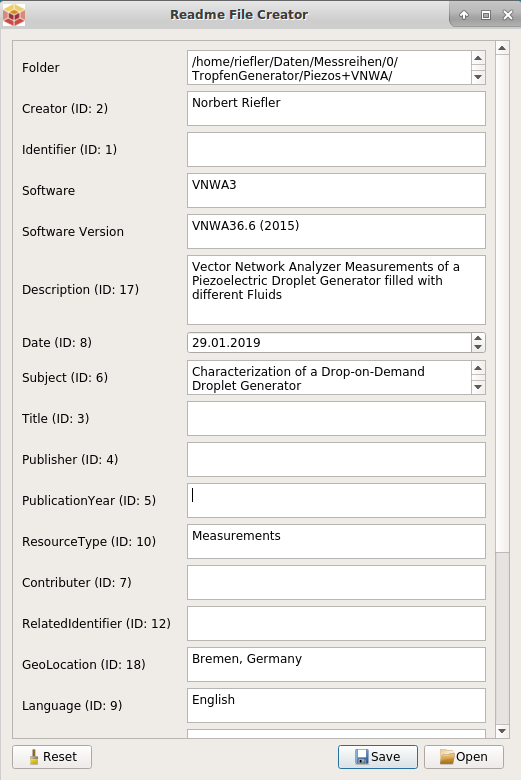
\includegraphics[width=\linewidth]{Figure02_ReadmeFileCreator.png}
	\caption{Data Input Tool: Readme-File-Creator}
	\label{fig:readme-creator}
\end{wrapfigure}
%
\textbf{ID 8: Date} \\
Key date associated with the data, e.g. project start, end date, data modification, data release date, or time period covered by the data \\[6pt]
%
\textbf{ID 9: Language} \\
Language(s) of the intellectual content of the resource, when applicable \\[6pt]
%
\textbf{ID 10: Resource Type} \\
A description of the resource; mostly ‘DataSet’, but may be ‘Audiovisual’, ‘High-Speed Images’, ‘DataPaper’, etc. \\[6pt]
%
\textbf{ID 19: Funding Reference} \\
Organizations or agencies who funded the research \\[6pt]
%
\textbf{ID 16: Rights} \\
Any known intellectual property rights held for the data. The best choice is either the Creative Commons license 'CC-BY' (BY attribution) or 'CC-0' for data and 'CC Version 4.0' for written documents. \\[6pt]
%
\textbf{ID 17: Description} \\
How the data was generated, including equipment or software used, experimental protocol, other things you might include in a lab notebook \\[6pt]
%
\textbf{ID 18: Geolocation} \\
When the data relates to a physical location, record information about its spatial coverage \\[6pt]
%


This tool displayed in figure \ref{fig:readme-creator} can be downloaded from the IWT-File-Server (see under $\rightarrow$Austausch $\rightarrow$Forschungs\-datenmanagement $\rightarrow$DataManagementGuidelines-ServiceFiles\linebreak$\rightarrow$ReadmeFileCreator) for every operating system to simplify metadata entry (figure on the right). You can create automatically a file called ‘readme.json’ with your metadata, embedded in a JSON (Java Scipt Object Notation) format, which is used as documentation as well as metadata for Data Science Methods. This file is stored in every directory which contains data or program code. Field entries can be empty if they are not applicable. \\
%
The same DataCite metadata structure can be included into the ELN (see chapter \ref{ssc:ELN}).



\subsection{Generation of a metadata scheme}
A schema is a logical plan showing the relationships between metadata elements,
normally through establishing rules for the use and management of metadata. An example of the development of a metadata schema is given in the paper of Elberskirch et al. \cite{elberskirch:2022}. There, all relevant parameters are collected to describe nanoparticles physically as well as biologically (toxicologically) in a comprehensive manner which yield a metadata scheme.
The development of suitable scheme for your specific domain can be helpful for structuring your data as well as your knowledge.





\section[Electronic Lab Notebook]{Electronic Lab Notebook (ELN)}\label{ssc:ELN}


\subsection{General information}

Electronic Lab Notebooks (ELNs) enable researchers to organize and store
experimental procedures, protocols, notes and data using their computer or
mobile device. ELNs can offer several advantages over the traditional paper
notebook in documenting research during the active phase of a project, including
searchability within and across notebooks, secure storage with multiple
redundancies, remote access to notebooks, and the ability to easily share
notebooks among team members and collaborators.

eLabFTW 
\includegraphics[height=9pt]{eLabFTW-logo3-ohneText.png} is an OpenSource, generic, browser based ELN, developed/initialized by
Nicolas Carpi (Institut Pasteuer, Paris) 2012. Data are stored in MySQL/MariaDB.
It is maintained by many developers and is used worldwide (Berkley, Indian
Institute of Technology, KIT, ...).
\begin{itemize}
  \item Access: \url{https://elabftw.iwt.zz/}
  \item Free definable status of the experiments (`finished', `running', ...)
  \item Definition of templates for a step-by-step procedure description of
        measurements
  \item Every experiment gets a unique ID and can be summarized easily as a pdf
  \item Free definable categories/tags
  \item Graphical text editor to describe your experiments and simulations
  \item File attachments of data with preview of common formats (pdf, tiff, png, …)
  \item Linking of experiments
  \item Time stamp service (RFC 3161, e.g. DFN)
  \item Data import/export (csv, zip, json, …)
  \item Access using, e.g., Python via an Application Programming Interface (API)
\end{itemize}


\subsection{IWT standard for documentation and structure}

To document scientific findings clearly and distinctly and trace them easily even after many years, the title and tags of an experiment or a simulation consists on a system shown in table \ref{table:tagging-system}. The information for ``material'', ``method'' and ``project'' or ``project abbrevation'' are abolutely imperative. You may also include more entries if required. The exactly same systematics are also applied for the tags (i.e. markers). The reason for this redundancy is the SQL database of eLabFTW which is much faster searching for tags.


\begin{table}[H]
 \centering
 \begin{tabular}{|p{5cm}|p{7cm}|p{3cm}|}
 \hline
 {\bf tags} & {\bf description} & {\bf examples} \\
 \hline
 \multicolumn{3}{|l|}{\bf mandatory information:} \\
 \hline
 material designation & DIN norm + material number; compositionin mass-\%  & 20MnCr5, TiO$_2$ \\ \hdashline
 project & project abbrevation, number, forerun& Aurora, IGF22777N, SPP2289 \\ \hdashline
 methods & analysing method, test method, process, simulation method & nitrifying, XRD, SOES, tensile test, UV-vis, OpenFOAM \\
 \hline
 \multicolumn{3}{|l|}{\bf optional information:} \\
 \hline
 device/system & label/name & DIL 805 A/D/T, PA7 \\ \hdashline
 sample label, sample number& for unique classification& 01-10036-22, E0165 \\ \hdashline
 base material, material type& chemical elements written-out& Iron, High entropy alloy, ceramic \\ \hdashline
 department & abbrevation like that of the team & WT-PA, VT-RST \\
 \hline
 %
 \end{tabular}
 \caption{Taging system with the always available tags for every experiment or simulation and the optional tags, which can be completely different according to the research domain.}
\label{table:tagging-system}
\end{table}



You have to create a pdf for every experiment (can be a simulation as well) simply by a click (`Make a pdf’) in the edit mode (see \texttt{‘04\_PrimaryData’} in Table   \ref{table:paper-directory-structure}) .This kind of documentation includes a unique QR-code and is required for data which is published! The QR-code enables a direct link to the data together with unique ID.

The \textbf{maximum size} of uploaded data should not exceed
\textbf{100Mbyte per file}. Further hints and tricks may be found in the eLab Wiki on the IWT NextCloud \footnote{https://nextcloud.iwt.zz/apps/collectives/ELN-Wiki-11} and in the eLab-document on the IWT file server ($\rightarrow$Austausch $\rightarrow$Forschungsdatenmanagement $\rightarrow$eLabFTW; please add comments there if you explore new ways of usage).


A template for the JSON field available in every experiment with entries for the metadata (see chapter \ref{sc:data-documentation}) is also saved on the IWT fileserver.


\section{Git Software repository}

Git 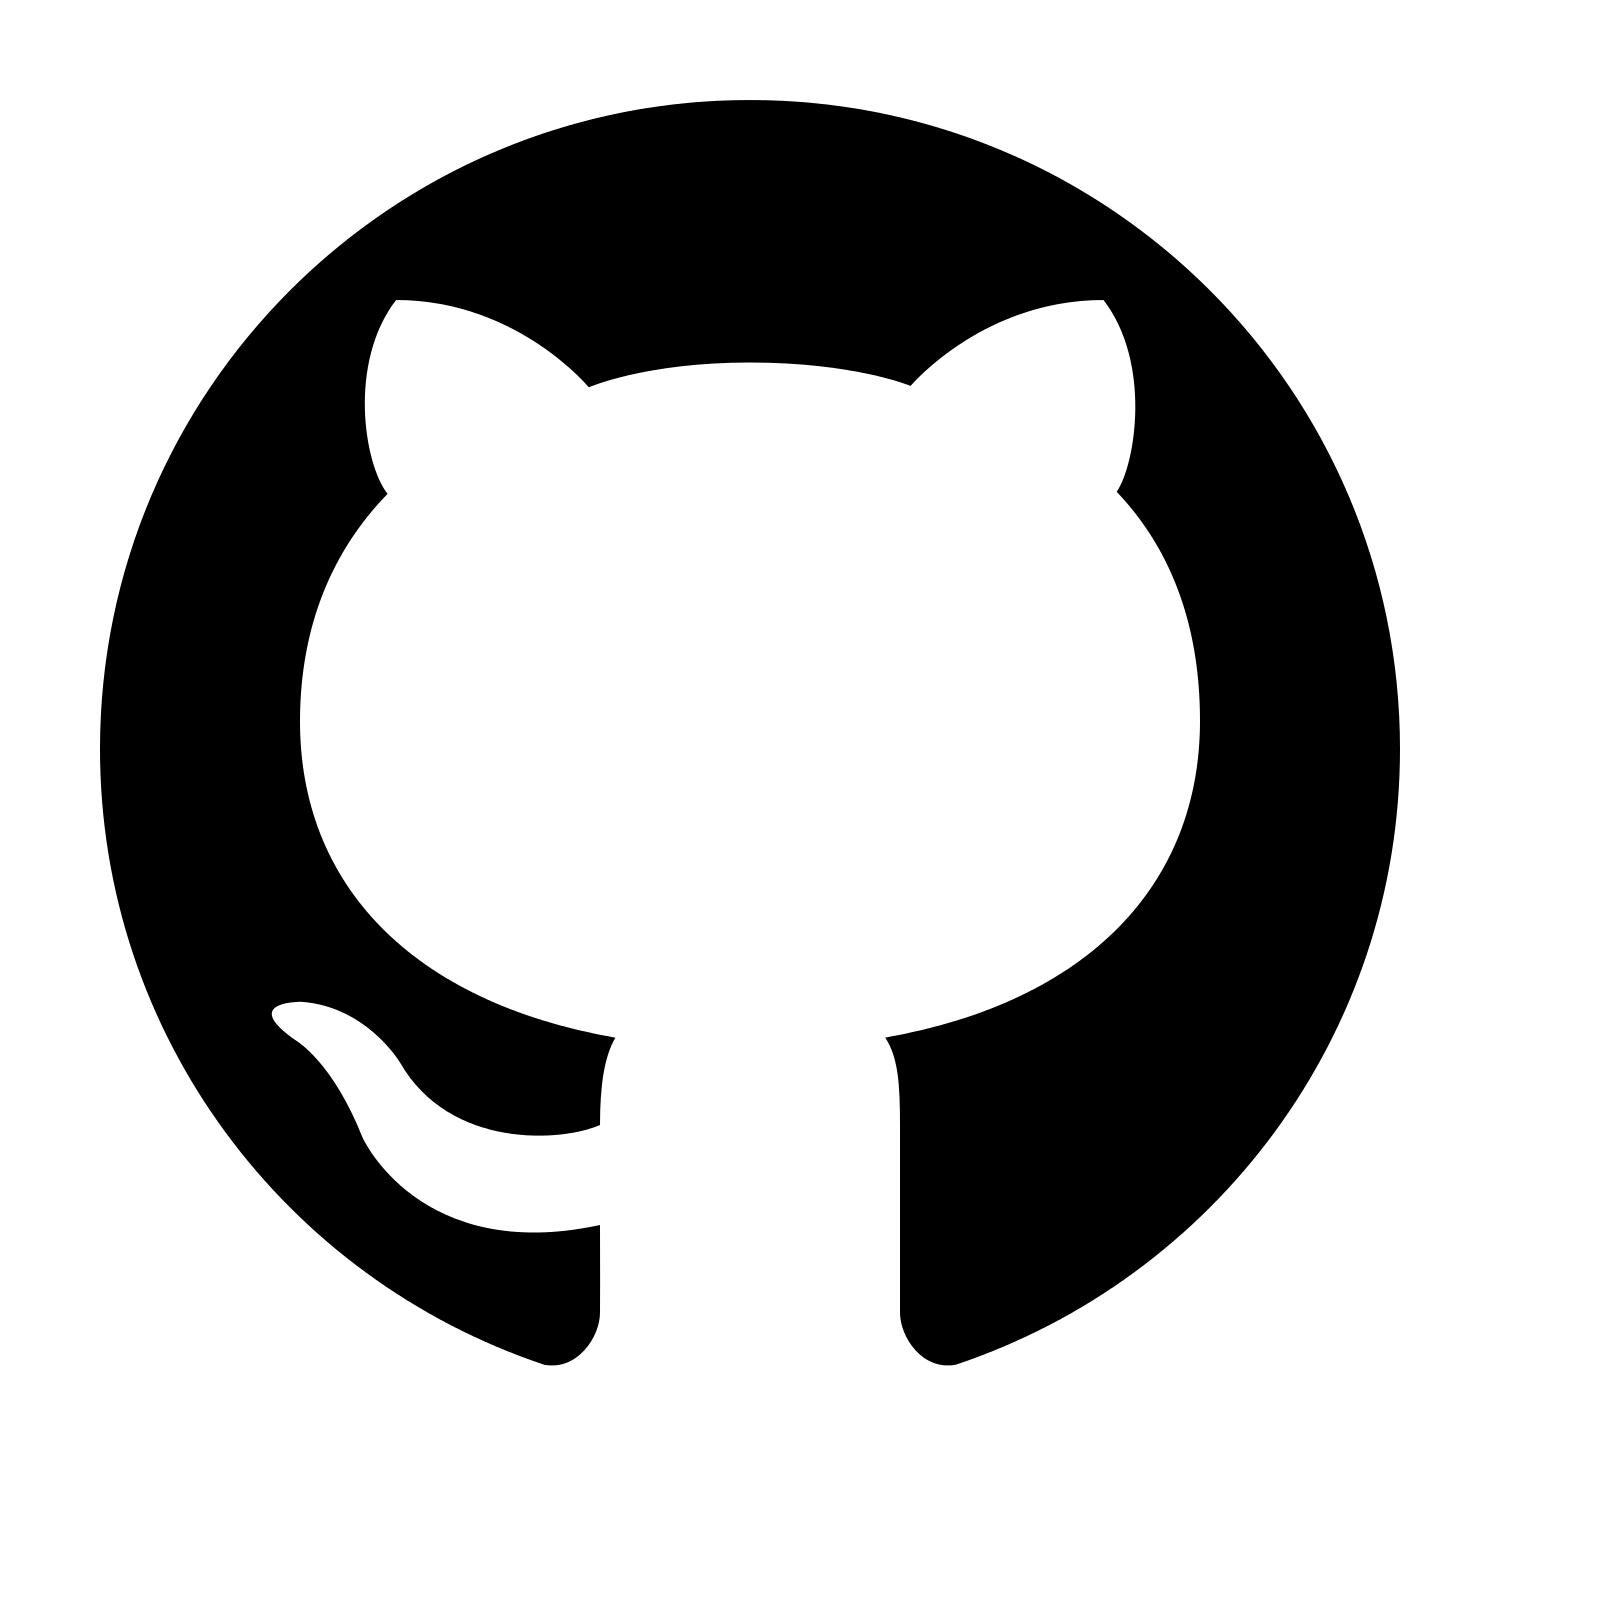
\includegraphics[height=9pt]{github-logo.png} is a web-based tool that provides a repository for the version control. It is used to manage, plan, create, verify and monitor your software developments. Furthermore, it can be used as a document versioning system. For example, during the creation of a larger piece of writing (a dissertation, papers, proposals, ...), you can enter the actual state of the document, and all the previous versions are stored as well. With that, every changed sentence can be tracked and reconstructed.

The L-IWT-Git can be accessed here: \url{https://github.com/Leibniz-IWT/}.
Registration via Email and Subject “IWT Organization access request” on:
\href{mailto:github@iwt.uni-bremen.de}%
{github@iwt.uni-bremen.de}


\section{FAIR Data and Open Science}\label{ssc:FAIR-Data}

FAIR (Findable, Accessible, Interoperable, Reusable) is a label for data which are findable in the Web, downloadable and can be used for own purposes. The data in the directory structure described in chapter \ref{ssc:data-for-publication} have to be stored in a FAIR way. This means that data from measurements must be clearly understandable (description of the used device with all adjustments, results with units as ASCII files, etc.) and data from simulations must be reproducible (source code, mesh, boundary conditions, etc.; no commercial programs, but their case file). This method also guarantees the fulfilment of Good Scientific Practice.

For all projects funded by public sponsors (and these are the prevailing case on L-IWT) there hold the principle that all gained data and developed methods have to be provided to the public. Therefore, the directory structure described above can be uploaded to zenodo \url{https://zenodo.org/}, a repository for scientific data, where you get a DOI for your data. But note: PDFs from a publisher can only be stored there if this is permitted explicitly by the journal and must be checked carefully. Usually, it is allowed to provide text and diagrams in an document formated by your own.

Data from other research institutes which are included in a publication, e.g. due to a cooperation, have to be saved FAIR according to our guidelines. This means they provide us their data (stored according to chapter  \ref{ssc:data-for-publication}). If they refuse this, they have to provide at least their data on a public repository.

The reuse of your data by others in the sense of the FAIR principles requires the link to a licence (without a statement the default term is "all rights reserved" which only allows viewing but no further usage).
%see https://academia.stackexchange.com/questions/63139/public-dataset-without-license-what-is-allowed
Therefore, common licences are the 'CC-BY' licence for text and  the '3-clause BSD' license (or 'BSD-3') for software.

The FAIR principles belong to Open Data and is one part within the framework of Open Science, with Open Access of scientific papers and Open Source of software as the three main components. Further information, including the Leibniz Open Science guidelines, can be found on the IWT webpage\footnote{https://www.iwt-bremen.de/en/institute/about-us/open-science}.





\subsection{Publishing Protocols, Data, and Code as Standalone Outputs}
\label{sec:standalone-outputs}

Research projects usually report their outcomes in one or two articles that focus
mainly on the methods and results. The collected data and the scripts written for the
analysis are treated as supplementary material and often stay unpublished. This often
hinders methodological transparency and independent reproducibility, and it limits
further use of the data and code.

IWT therefore encourages treating research methods, datasets, and codebases as separate
research outputs. If possible, each should be published with documentation, ideally as
a short paper, and stored and documented according to these guidelines: the directory
structure in \autoref{ssc:data-for-publication}, metadata in \autoref{ssc:Doku+Metadata}, ELN records with QR codes in \autoref{ssc:ELN}, and licenses as described above. These papers act as guides to the associated
resources. They can be published at different stages of a project, which also shows its
progress. The main benefits are:

\begin{enumerate}
	\item \textbf{Protocol paper or pre-registration.} If you publish your methodology
	and analysis plan before starting the analysis, either as a pre-registration or as a
	protocol paper (also known as registered protocols), you formally state your
	hypotheses or core idea and research plan. You can then get feedback and revise the
	plan if needed. This protects against p-hacking, hypothesizing after the results are
	known (HARKing), and other questionable research practices.
	\item \textbf{Data paper.} A curated dataset with metadata is a valuable resource
	that can often support studies beyond your own. Publishing it with a data paper makes
	it easier for others to reproduce or validate your findings and to reuse the dataset
	in their own work.
	\item \textbf{Software paper.} Publishing your codebase or analysis pipeline with a
	software paper makes your methods and analysis fully transparent and lets others
	adapt your code for their own projects.
	\item \textbf{Citability and visibility.} Publishing these outputs as research papers
	with DOIs, or alongside them, makes them visible and citable milestones. Platforms
	such as Google Scholar, ResearchGate, Scopus, and Semantic Scholar track citations of
	these papers, which they often do not do for data or code repositories alone, even
	when those have DOIs.
\end{enumerate}

Researchers interested in this approach can set up an internal collaboration with the
Digital Technologies (DT) department. DT helps develop a concrete publication plan for
the project and shares the work of preparing and publishing these materials. For
details, contact Prof. Dr. Evgeniya Kabliman.\footnote{%
	\url{https://share.iwt-bremen.de/s/nFxcb6raDN49eYx}
	(Password: \texttt{Open\_2026!})}
\section{EndNote}

We have EndNote as literature management software for everyone (single user
system). EndNote can be integrated into Word to manage cited references in
publications. It also serves as a literature database for papers, textbooks,
presentations etc. And it is used as the literature database for all
publications from the IWT.

\section{Further Tools for Data Management}

\begin{itemize}
  \item Search for Data Repositories: \url{https://www.re3data.org/}
  \item \url{https://zenodo.org/}  $\rightarrow$ scientific data, publications,
        reports, presentations, videos, etc.
  \item \url{https://www.ukdataservice.ac.uk/manage-data/format/recommended-formats}
        \begin{itemize}
          \item[$\rightarrow$] list of recommended data formats
        \end{itemize}
  \item \url{http://rd-alliance.github.io/metadata-directory/standards/}
        $\rightarrow$ Metadata Discipline Standard Formats
  \item Renaming Tools: PSRenamer, ExifToolGUI
\end{itemize}


\appendix
\addcontentsline{toc}{section}{Bibliography}
\printbibliography

\pagebreak


\section{Appendix}



\subsection{How to Store Papers – `Dummy Paper'}\label{app:dummy-paper}

The following screenshot shows a complete data structure of a dummy paper.
You may find this dummy paper on our IWT file server under $\rightarrow$Austausch $\rightarrow$For\-schungsdatenmanagement $\rightarrow$Data\-Manage\-mentGuidelines-ServiceFiles  $\rightarrow$DummyPaper. Basically, the idea is that every data in the
paper, whether it is a figure or a table, can be related to the original source
of the measurement or the simulation. This is realized in the Dummy Paper by
Matlab scripts, but can be done using other means as well (Python, Excel). The
point is: No matter how, but you have to give a relation between the data saved
in the \texttt{‘04\_PrimaryData’} directory and their representation in the
publication. All figures and their generating scripts – here Matlab files – are
given together with the measurement data so that running a Matlab (Octave)
script within that directory generates the according figure. In the end, someone
else can reproduce your results given in your publication. In case of other data
like SEM images for instance, you can refer to them by a PDF generated by the
ELN including a link to the experiment stored there.

\begin{figure}[H]
	\centering
	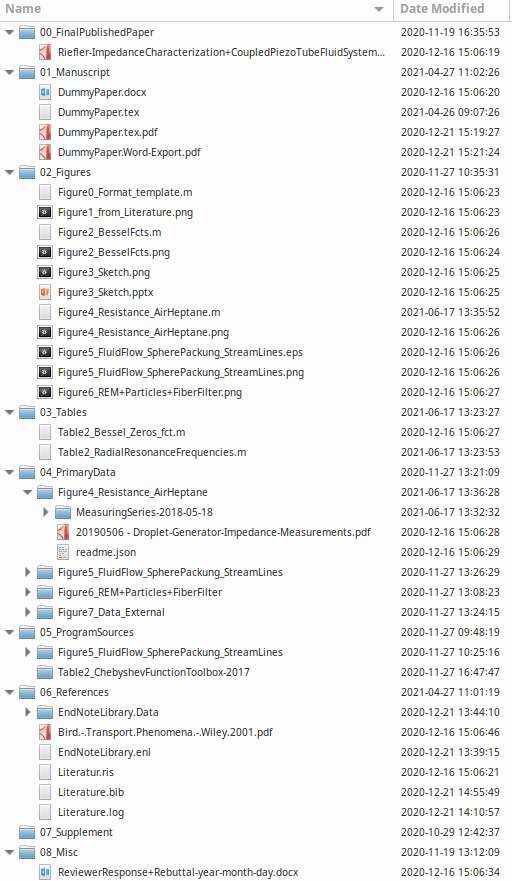
\includegraphics[
	width=0.45\linewidth,
	height=0.5\textheight,
	keepaspectratio
	]{Figure03_DummyPaperStructureExample4.png}
	\caption{Complete data structure of a dummy paper.}
	\label{fig:dummy-paper}
\end{figure}

The `Dummy Paper' contains a Word and a LaTeX template in
\texttt{‘01\_Manuscript’}. The EndNote or BibTeX literature references are in
\texttt{‘06\_References’}. Both, the EndNote file ‘*.enl’ or the BibTeX file
‘*.bib’, should include links between the references and the freely accessible
PDFs of the papers and books also saved in \texttt{‘06\_References’}.

\subsection{How to Write a DMP}

\subsubsection{Motivation}

The handling of the data, created during a project, contains several issues
which are described in a Data Management Plan (DMP). A DMP contains structured
information about the research process of the corresponding project. But these
information has to be given long before a project is started: Applicants have
to create a DMP in every proposal, required by all important research funding
organizations (DFG, BMBF, etc.). So in the process of writing, applicants start
to think about how they will treat data. The following topics belongs to typical
DMPs and might be of interest to you; more details can be found in
\cite{dfg2021,hannover2020}:
\begin{enumerate}
	\item Administrative information: project name, kind of funding, time period.
	\item Methods of data generation: simulations, experiments (devices),
	data size, kind of data documentation.
	\item Data safety: location, interval and capacity of storage device,
	who gets access.
	\item Archiving: which data are archived where with what kinds of metadata.
	\item Data sharing: which repository, license condition, required metadata.
	\item Resources and responsibility: who is responsible for processes, IT,
	defining defaults and formats, monitoring; required personal resources;
	costs.
\end{enumerate}
Please see \cite{dfg2021,hannover2020} for more details; some exemplary DMPs can be found here:
\url{https://www.cms.hu-berlin.de/de/dl/dataman/arbeiten/dmp_erstellen}



\subsubsection{Elements of a DMP}

There is no unified structure of DMPs due to the vast number of different
research tasks. In the following, the main elements of a DMP from the
TIB Hannover are listed, which can be found also in the recommendation of the
DFG\footnote{\url{https://www.dfg.de/download/pdf/foerderung/grundlagen_dfg_foerderung/forschungsdaten/forschungsdaten_checkliste_de.pdf}}

\begin{enumerate}[start=0, label=\textbf{\arabic*})]
  \item \textbf{Administrative information}
        \begin{itemize}
          \item Project name
          \item Project participants
          \item Project description
          \item Project ground (doctorate, third party funding, etc.)
          \item Project duration
          \item Version of this DMP
        \end{itemize}
  \item \textbf{Methods and kinds of data gathering}
        \begin{itemize}
          \item Are there primary data generated, or will be secondary data used?
          \item Which data types / formats are generated and processed?
          \item How large are the data?
          \item Which equipment (instruments, hardware, software, etc.)
                will be used?
          \item How are the data organized? (Directory of file oriented
                structure? Version control?)
          \item How is the research process and the data been documented?
          \item Which (technical) standards will be used for
                description/documentation (metadata, classification)?
          \item How are the metadata been generated (e.g. automatically,
                manually, after a guideline, self-defined)?
        \end{itemize}
  \item \textbf{Backup and data safety}
        \begin{itemize}
          \item Where are the data stored?
          \item Which capacity is required?
          \item Interval of data safety?
          \item Are there any protective measures required for sensitive data?
          \item Are there any third party of project partners (e.g. in joint
                projects) who need access to the data?
        \end{itemize}
  \item \textbf{Archiving}
        \begin{itemize}
          \item Which data is archived?
          \item On which data carrier?
          \item Are there any requirements for the operators of the
                infrastructure? E.g. data curation?
          \item Which metadata have to be provided to find the archived data?
          \item Which information is additionally required to understand the
                context of the data?
          \item How long are the data archived?
          \item Are there any legal technicalities for the data archiving?
          \item What are the costs for which service?
        \end{itemize}
  \item \textbf{Data sharing and publication}
        \begin{itemize}
          \item Are there data which must be shared with others?
          \item What are the possible systems for data sharing?
          \item Which metadata and documentation are additionally required for
                third parties to use the data?
          \item Where (data repository, data journal) will the data be
                published, and how (e.g. open access, with embargo time,
                restricted access)?
          \item What are the license condition for the published data?
                (E.g. `CC BY 4.0')
        \end{itemize}
  \item \textbf{Resources and responsibilities}
        \begin{itemize}
          \item How is the distribution of responsibility governed in this project?
          \item How is responsible for the data management (processes, IT,
                guidelines, formats, monitoring)?
          \item Required personal resources for a successful
                implementation/realization?
          \item What are the costs within the project phase and
                possibly thereafter?
          \item Which infrastructure resources are required, with additionally
                costs?
        \end{itemize}
\end{enumerate}




\pagebreak
\subsection{Glossary}

\begin{table}[h]
\begin{tabular}{lll}
AiF   & $\ldots$  & Arbeits�gemeinschaft industrieller Forschungs�vereinigungen \\
ASCII & $\ldots$  & American Standard Code for Information Interchange \\
BMBF  & $\ldots$  & Bundesministerium f�r Bildung und Forschung \\
BSD   & $\ldots$  & Berkeley Software Distribution \\
CC-BY & $\ldots$  & Creative Commons - BY attribution \\
DFG   & $\ldots$  & Deutsche Forschungs-Gemeinschaft \\
DMP   & $\ldots$  & Data Management Plan \\
ELN   & $\ldots$  & Elektronic Laboratory Notebook \\
ERC   & $\ldots$  & European Research Council \\
FAIR  & $\ldots$  & Findable Accessible Interoperable Reusable \\
GWP   & $\ldots$  & Gute Wissenschaftliche Praxis \\
ISO   & $\ldots$  & International Organization for Standardization  \\
JSON  & $\ldots$  & Java Script Object Notifier \\
NAS   & $\ldots$  & Network Access Storage \\
XML   & $\ldots$  & eXtended Markup Language \\

\end{tabular} {lll}
\end{table}




\subsection*{Acknowledgement}
This document is grown over the years during long discussions within the Leibniz-IWT, but also outside through many thoughts from the research data management community like the NFDI consortia MatWerk \footnote{\url{https://nfdi-matwerk.de/}} or the joint project Plattform MaterialDigital \footnote{\url{https://www.material-digital.de/}}. Last, the help and contribution of Tamara Engoian and Niloy Sikder are gratefully acknowledged.



\end{document}
